% !TEX program = XeLaTeX
% !TEX encoding = UTF-8
\documentclass[UTF8,nofonts]{article}
%{ctexart}


%\setCJKmainfont[BoldFont=FandolSong-Bold.otf,ItalicFont=FandolKai-Regular.otf]{FandolSong-Regular.otf}
%\setCJKsansfont[BoldFont=FandolHei-Bold.otf]{FandolHei-Regular.otf}
%\setCJKmonofont{FandolFang-Regular.otf}

\usepackage[brazilian]{babel}
\usepackage[T1]{fontenc}
\usepackage[utf8x]{inputenc}
\usepackage{url}
\usepackage{lipsum}
\usepackage{cancel}
\usepackage{xspace}
\usepackage{graphicx}
\usepackage{multicol}
\usepackage{multirow}
\usepackage{subfig}
\usepackage{amsmath}
\usepackage{amssymb}
\usepackage[a4paper, width=186mm, top=18mm, bottom=18mm, includeheadfoot]{geometry}
%\usepackage[a4paper, width=140mm, top=18mm, bottom=22mm, includeheadfoot]{geometry}
\usepackage{booktabs}
\usepackage{array}
\usepackage{verbatim}
\usepackage{caption}
\usepackage{natbib}
\usepackage{booktabs}
\usepackage{float}
\usepackage{pdflscape}
\usepackage{mathtools}
\usepackage[usenames, dvipsnames]{xcolor}
\usepackage{afterpage}
\usepackage{pgf}
\usepackage{tikz}
\usepackage{dirtree}
\usepackage[style=american]{csquotes}
\usepackage{amsfonts}
\usepackage{tikz}
\usepackage{tkz-graph}
\usetikzlibrary{arrows,decorations.pathmorphing,automata,positioning,backgrounds,fit,shapes.symbols,chains,intersections}

\newtheorem{definition}{Definition}[section]
\newtheorem{theorem}{Theorem}[section]
\newtheorem{lemma}{Lemma}
\newtheorem{proof}{Proof} [section]



\usepackage[toc, page, title, titletoc, header]{appendix}
\usepackage{marginnote}
\usepackage{tablefootnote}

%\renewcommand\appendixname{附\ 录}
%\renewcommand\appendixpagename{附\ 录}
%\renewcommand\appendixtocname{附\ 录}
\renewcommand\abstractname{Abstract}


\usepackage{perpage} %the perpage package
\MakePerPage{footnote} %the perpage package command

\usetikzlibrary{shapes.geometric}%
\usepackage{color}
%\usepackage[pages=some, placement=top]{background}
\usepackage{eso-pic}
\usepackage[final]{pdfpages}

%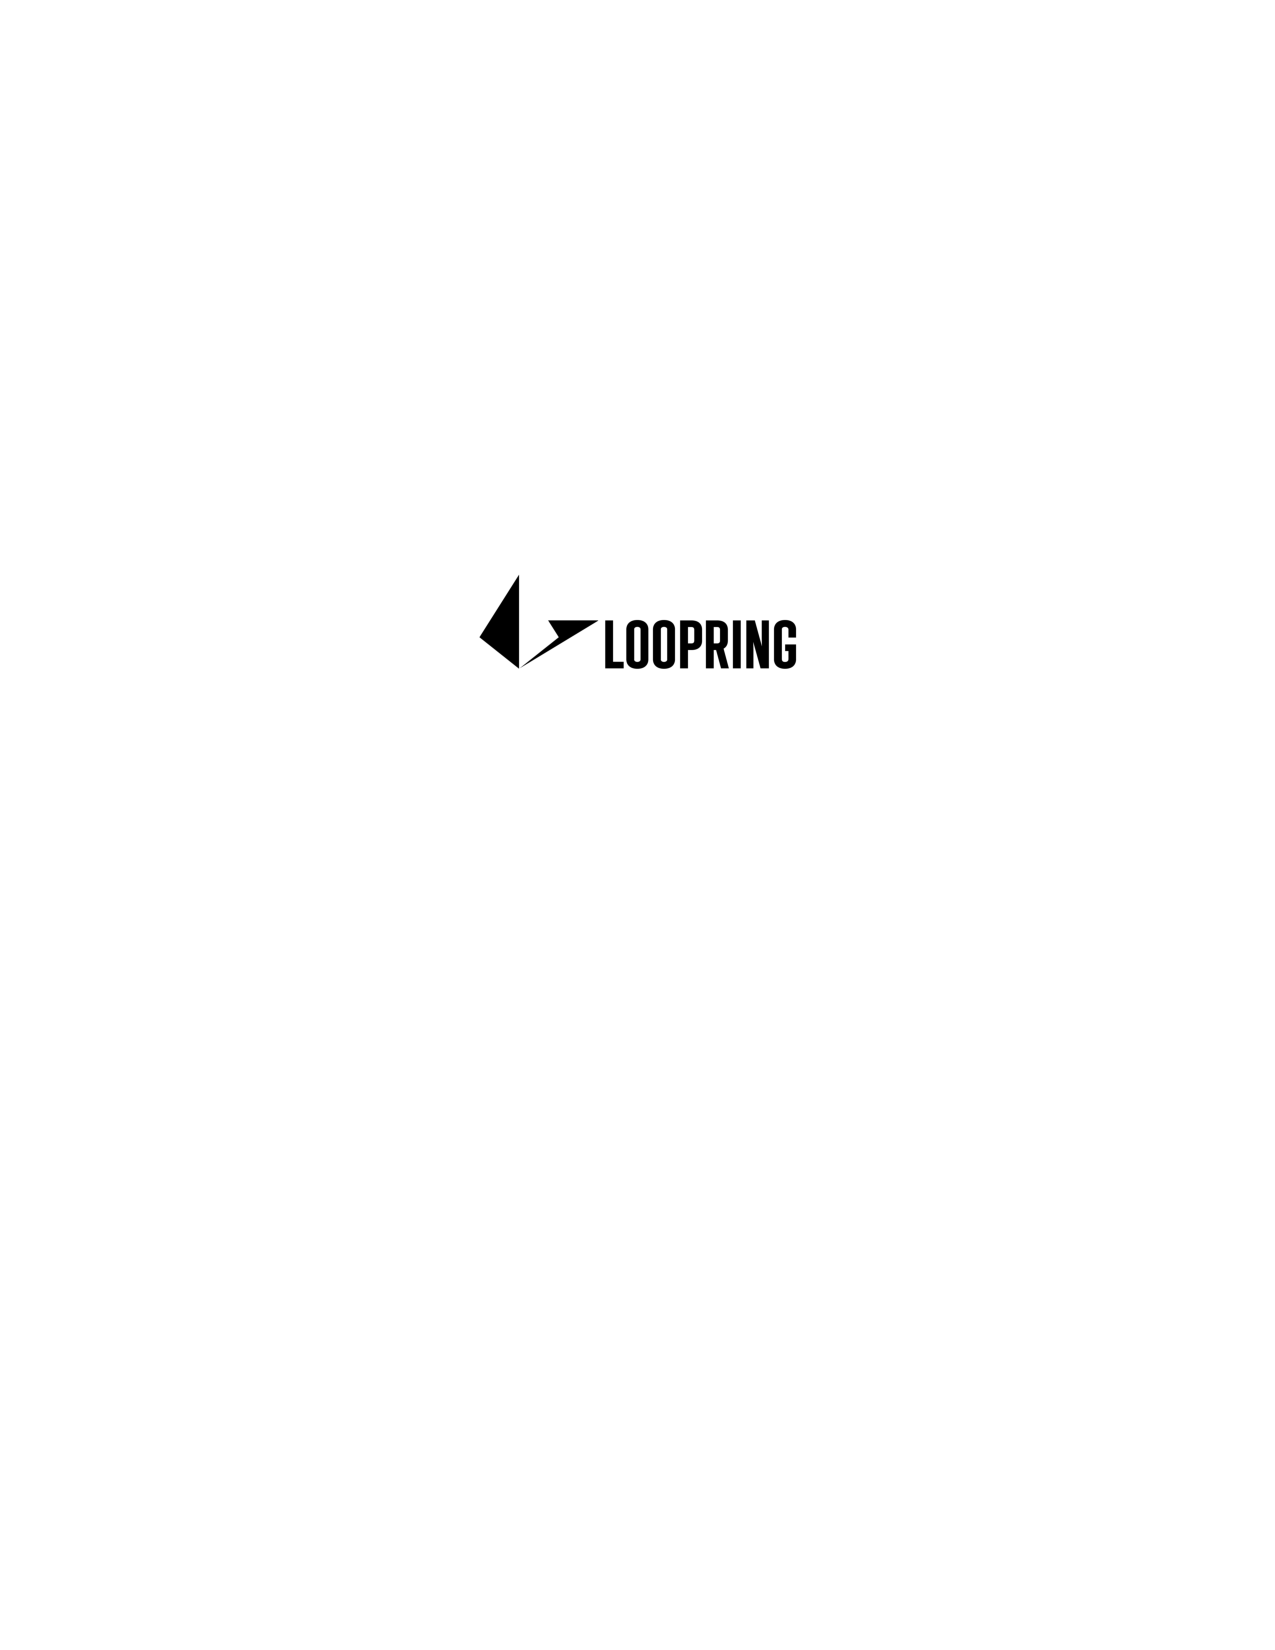
\includepdf[pages=1]{cover}
\hyphenpenalty=750

\title{\textbf{Loopring:}\\\textbf{Um Protocolo de Câmbio de Tokens Descentralizado}}
\author{
  Daniel Wang\\
  \texttt{daniel@loopring.org}\\
  \and
  	Jay Zhou\\
  	\texttt{jay@loopring.org}\\
  	\and
  	Alex Wang\\
  	\texttt{alex@loopring.org}\\
  	\and
  	Matthew Finestone\\
  	\texttt{matt.finestone@gmail.com}\\ 
  \\
  \texttt{https://loopring.org}
 }

\makeatletter
\def\CTEX@section@format{\Large\bfseries}
\makeatother

\makeatletter
\newenvironment{tablehere}
 {\def\@captype{table}}
 {}

\newenvironment{figurehere}
 {\def\@captype{figure}}
 {}
\makeatother
%
%\newcommand\BackgroundPic{%
%\put(0, 0){%
%\parbox[b][\paperheight]{\paperwidth}{%
%\vfill
%\centering
%\includegraphics[width=\paperwidth, height=\paperheight, %
%%keepaspectratio]{images/background.jpg}%
%]{images/background.jpg}%
%\vfill
%}}}


\begin{document}
%\AddToShipoutPicture{\BackgroundPic}
\maketitle


\begin{abstract}
O Loopring é um protocolo aberto para a construção de câmbios descentralizados. O Loopring opera como um conjunto público de contratos inteligentes responsáveis pelo comércio e liquidez, com um grupo de agentes em cadeia que agregam e comunicam pedidos. O protocolo é gratuito, extensível e serve como um módulo estrutural padronizado para aplicativos descentralizados (dApps) que incorporam a funcionalidade de câmbio. Seus padrões interfuncionais facilitam a negociação ainda que ela seja anônima e não seja digna de confiança. Uma importante melhoria em relação aos atuais protocolos de câmbio descentralizado é a capacidade de que os pedidos sejam misturados e combinados com outros diferentes pedidos, eliminando assim as restrições dos pares de comercialização de dois tokens e melhorando consideravelmente a liquidez. O Loopring também utiliza uma solução única e sólida para evitar o front running: a tentativa desleal de enviar transações para um bloco mais rapidamente do que o provedor original da solução. O Loopring é independente do blockchain, além de ser aplicável em qualquer blockchain com a funcionalidade de contrato inteligente. No momento da escrita, ele é operável em Ethereum  \cite{buterin2017ethereum} \cite{wood2014ethereum} e Qtum \cite{dai2017smart} com NEO \cite{atterlonn2018distributed} em construção.
\end{abstract}



\begin{multicols}{2}
\section{Introdução\label{sec:introduction}}


Com a multiplicação de ativos baseados no blockchain, a necessidade de trocar esses ativos entre as contrapartes aumentou significativamente. À medida que milhares de novos tokens são introduzidos – incluindo a tokenização de ativos tradicionais – essa necessidade é ampliada. Seja o câmbio de tokens por motivações especulativas de negociação, ou conversão para o acesso de redes através de seus tokens de utilidade nativos, a capacidade de trocar um ativo cripto por outro é fundamental para um ecossistema maior. 

De fato, existe uma energia potencial em ativos  \cite{desotocapital}, e a compreensão dessa energia - de capital de desbloqueio - requer não apenas a propriedade, que os blockchains permitiram invariavelmente, mas também a capacidade de transferir e transformar gratuitamente esses ativos.
 
Como tal, o câmbio de tokens sem confiança (valor) é um caso de uso convincente para a tecnologia blockchain. Até agora, no entanto, os entusiastas da criptografia decidiram maioritariamente por tokens de negociação em câmbios centralizados tradicionais. O protocolo Loopring é necessário uma vez que, assim como o Bitcoin  \cite{nakamoto2008bitcoin} destacou enfaticamente isso, em relação ao dinheiro eletrônico peer-to-peer, “os principais benefícios são perdidos se um terceiro de confiança ainda for necessário para evitar o gasto duplo”, e assim também são os principais benefícios dos ativos descentralizados perdidos, caso eles precisem passar por trocas confiáveis, fechadas e centralizadas.Negociar tokens descentralizados em câmbios centralizados não faz sentido do ponto de vista filosófico, uma vez que essa negociação não consegue sustentar as virtudes adotadas por esses projetos descentralizados. 
Existem também inúmeros riscos práticos e limitações no uso de câmbios centralizados, descritos abaixo. Os câmbios descentralizados (DEXs) \cite{schuh2015bitshares} \cite{bancor} \cite{kyber} procuraram abordar tais questões e, em muitos casos, conseguiram aliviar os riscos de segurança utilizando os blockchains para a desintermediação. No entanto, na medida em que a capacidade do DEX torna-se uma infraestrutura fundamental para a nova economia, há espaço substancial para a melhoria do desempenho. O Loopring tem como objetivo fornecer ferramentas modulares para essa infraestrutura com seu protocolo aberto independente do dApp.


\section{Panorama de Câmbio Vigente\label{sec:current_exchange_landscape}}

\subsection{Inadequações dos Câmbios Centralizados}
Os três principais riscos das câmbios centralizados são; 1) Falta de segurança, 2) Falta de transparência e 3) Falta de liquidez.

\textbf{A falta de segurança:} é proveniente do fato de que usuários geralmente entregam o controle de suas chaves privadas (fundos) a uma entidade centralizada. Isso expõe os usuários à possibilidade de que os câmbios centralizados sejam vítimas de invasores (hackers) mal-intencionados. Os riscos de segurança e invasão que defrontam todos os câmbios centralizados são bem conhecidos \cite{coincheckhack}  \cite{mcmillan2014inside}, mas muitas vezes são aceitos como “Estacas da Tabela” para negociação de token. Os câmbios centralizados continuam a ser alvos fáceis para os ataque de hackers, uma vez que seus servidores custodiam milhões de dólares em fundos de usuários. Os desenvolvedores do câmbio também podem cometer erros acidentais, mas sem más intenções, com os fundos do usuário. De maneira simples, os usuários não estão no controle de seus próprios tokens quando depositados em um câmbio centralizado.
.

\textbf{A falta de transparência:} expõe os usuários ao risco de câmbios desleais que atuam de forma injusta. A distinção aqui é pelas más intenções do operador de câmbio, já que os usuários não estão realmente negociando seus próprios ativos em câmbios centralizados, mas sim um IOU. Quando os tokens são enviados para a carteira do câmbio, esse câmbio fica sob custódia e oferece um IOU em seu lugar. Todos os negócios são, de forma efetiva, entre os IOUs dos usuários.  Para retirar, os usuários resgatam seus IOUs com o câmbio e recebem seus tokens em seu endereço da carteira externa. Ao longo desse processo, existe uma falta de transparência, e o câmbio pode ser interrompido, congelar sua conta, ir à falência, etc. Também é possível que eles usem ativos de usuário para outros fins enquanto estão sob custódia, como emprestá-los a terceiros. A falta de transparência não quer dizer que os usuários perderá todos os seus fundos, mas pode acarretar em altas taxas de negociação, atrasos quando houver alta demanda, riscos com regulamentações e pedidos em execução.

\textbf{Falta de Liquidez:} Do ponto de vista dos operadores de câmbio, a liquidez fragmentada inibe a entrada de novas trocas por causa de dois cenários de “o vencedor-leva-tudo”. Primeiro, o câmbio com o maior número de pares negociáveis ganha, tendo em vista que os usuários acham isso necessário para conduzir todos os seus negócios em um intercâmbio. Em segundo lugar, o intercâmbio com o maior registro de pedidos vence, devido a spreads de oferta-procura favoráveis para cada par de negociação. Isso desencoraja a concorrência dos iniciantes, uma vez que é difícil para eles acumularem liquidez inicial.
Como resultado, muitas trocas geram uma alta participação de mercado, apesar das reclamações dos usuários e até mesmo das grandes incidências de hackers.

Vale a pena notar que, à medida que as centrais ganham quota de mercado, elas se tornam um alvo cada vez maior dos invasores


Do ponto de vista dos usuários, a liquidez fragmentada reduz significativamente a experiência do usuário. Em um câmbio centralizado, os usuários só podem negociar dentro dos próprios conjuntos de liquidez do câmbio, mediante seu próprio registro de pedidos e entre seus pares de token suportados. Para trocar o token \verb|A| pelo token \verb|B|,  os usuários devem ir para um câmbio que ofereça suporte para ambos os tokens, ou devem se registrar em diferentes trocas, divulgando informações pessoais. Os usuários geralmente precisam executar negociações preliminares ou intermediárias, normalmente mediante ao BTC ou a ETH, pagando spreads de oferta-procura no processo. Finalmente, os registros de pedidos podem não ser suficientemente profundos para concluir o negócio sem um deslize relevante. Mesmo que o câmbio pretenda processar grandes volumes, não há garantia de que esse volume e liquidez não sejam falsos.\cite{fakevolume}.


O resultado são silos de liquidez desconexos e um ecossistema fragmentado que se assemelha ao legado sistema financeiro, com volume de negociação significativo centralizado em poucas trocas. As promessas de liquidez global de blockchains não têm mérito dentro de câmbios centralizados.

\subsection{Inadequações dos Antigos Câmbios Descentralizados}
Os câmbios descentralizados diferem dos câmbios centralizados em parte porque os usuários mantêm o controle de suas chaves privadas (ativos) executando negociações diretamente no blockchain subjacente. Aproveitando a tecnologia confiável de criptomoedas, eles por si só mitigam com sucesso muitos dos riscos acima mencionados relacionados à segurança. No entanto, problemas em relação ao desempenho e limitações estruturais persistem.

A liquidez muitas vezes continua sendo um problema, visto que os usuários devem buscar contrapartes em diferentes conjuntos e padrões de liquidez. Os efeitos de liquidez fragmentada estão presentes se os DEXs ou os dApps de forma geral não empregarem padrões consistentes para interoperar, e se os pedidos não forem compartilhados/propagados em uma rede ampla. A liquidez dos registros de pedidos limitados e, especificamente, sua resiliência -- a rapidez com que os pedidos limitados são regeneradas -- podem afetar significativamente as devidas estratégias de negociação\cite{limitorderliquidity}.A ausência de tais padrões resultou não apenas na redução da liquidez, mas também em exposição a uma série de contratos inteligentes de propriedade potencialmente incertos. 


Além disso, como as negociações são realizadas na cadeia, os DEXs herdam limitações do blockchain subjacente, a saber: escalabilidade, atrasos na execução (mineração) e modificações de custos elevados para pedidos. Assim, os registros de pedidos de blockchain não são particularmente adequados, já que a execução de código no blockchain incorre em um custo (gás), tornando as cadências de cancelamento de pedidos múltiplas inviavelmente caras. 

Finalmente, considerando que os registros de pedidos de blockchain sejam públicos, a transação para fazer um pedido é visível pelos mineradores na medida em que aguarda ser extraída para o próximo bloco e colocada em um registro de pedidos. Esse atraso expõe o usuário ao risco de estar na frente e ter o preço ou a execução se movendo contra ele.


\subsection{Soluções Híbridas}
Pelas razões acima, câmbios totalmente baseados em blockchain têm limitações que os tornam pouco competitivos com câmbios centralizados. Há uma troca entre a confiabilidade inerente em cadeia e a velocidade do intercâmbio centralizado e a flexibilidade do pedido. Protocolos como Loopring e 0x  \cite{warren20170x} estendem uma solução de estabelecimento em cadeia (on-chain) com o gerenciamento de pedidos fora da cadeia (off-chain). Essas soluções giram em torno de contratos inteligentes abertos, mas navegam nas limitações de escalabilidade, executando várias funções off-chain e dando aos nós flexibilidade no cumprimento de funções críticas para a rede. No entanto, os contras permanecem também para o modelo híbrido \cite{costofdecent}. O protocolo Loopring propõe diferenças significativas em nossa abordagem para uma solução híbrida ao longo deste artigo.

\section{Protocolo de Loopring\label{sec:loopring_protocol}}
O Loopring não é um DEX, mas um protocolo modular para construir DEXs em vários blockchains. Desmontamos as partes componentes de um câmbio tradicional e oferecemos um conjunto de contratos públicos inteligentes e agentes descentralizados em seu lugar. As funções na rede incluem carteiras, relés, blockchains de consórcio de compartilhamento de liquidez, navegadores de pedidos de compras, Ring-Miners e serviços de tokenização de ativos. Antes de definir cada um, devemos primeiro entender os pedidos de Loopring.

\subsection{Anel de Pedido (Order ring)\label{sec:order_ring}}
Os pedidos de loopring são expressos no que chamamos de Modelo de Pedido Unidirecional (UDOM) \cite{coinport2014udom}. A UDOM expressa pedidos como solicitações de troca de tokens, \verb|montanteS|/\verb|montanteB|, (valor para vender/comprar) em vez de licitações e pedidos. Como cada pedido é apenas uma taxa cambial entre dois tokens, um recurso poderoso do protocolo é a mistura e correspondência de vários pedidos no comércio circular. Utilizando até 16 pedidos em vez de um único par de negociação, há um aumento significativo na liquidez e potencial para melhoria de preço.


\begin{center}
\begin{figurehere}
\centering
\tikzstyle{block} = [draw, fill=blue!20, rectangle, 
    minimum height=3em, minimum width=6em]
\tikzstyle{sum} = [draw, fill=blue!20, circle, node distance=1cm]
\tikzstyle{input} = [coordinate]
\tikzstyle{output} = [coordinate]
\tikzstyle{pinstyle} = [pin edge={to-,thin,black}]

\begin{tikzpicture}[
    auto, 
    node distance=2cm,
    >=latex',
    font=\bfseries\footnotesize\sffamily,
    order/.style={
		scale=0.7,
		rectangle,
		rounded corners,
		draw=black, 
		text centered,
%		text width=5cm,
		minimum height=12mm,
		fill=white
	},
	label/.style={
		scale=0.7
	}
  ]
    % We start by placing the blocks

  \node [order] (order2) 
 {%
 \begin{tabular}{l}
  \textbf{ORDEM\#2}\\
  \textbf{Proprietário: Y}\\
  \textbf{MontanteS: 9B}\\
  \textbf{MontanteB: 12C}
 \end{tabular}
 };
 
  \node [order, below of=order2, xshift=-3.5cm] (order1) 
 {%
 \begin{tabular}{l}
  \textbf{ORDEM\#1}\\
  \textbf{Proprietário: X}\\
  \textbf{MontanteS: 10000A}\\
  \textbf{MontanteB: 2B}
 \end{tabular}
 };
 
 
  \node [order, below of=order2, xshift=3.5cm] (order3) 
 {%
 \begin{tabular}{l}
  \textbf{ORDEM\#3}\\
  \textbf{Propietário: Z}\\
  \textbf{MontanteS: 100C}\\
  \textbf{MontanteB: 160A}
 \end{tabular}
 };
 
 \draw [draw,->] (order1) -- node [label] {\textbf{7898A}} (order3);
 \draw [draw,->] (order2) -| node [label, xshift=-1.8cm] {\textbf{8B}} (order1);
 \draw [draw,->] (order3) |- node [label, xshift=1cm, yshift=0.24cm] {\textbf{98C}} (order2);

\end{tikzpicture}

\caption{Um anel de pedidos de 3 Pedidos}
\label{fig:ring}
\end{figurehere}
\end{center}



A figura acima mostra um anel de pedidos de 3 pedidos. O token de cada pedido para vender (\verb|tokenS|) é o token de outro pedido para comprar (\verb|tokenB|).Ele cria um loop que permite que cada pedido troque seus tokens desejados sem exigir um pedido oposto para seu par. As negociações tradicionais de pares de pedidos podem, é claro, ainda ser executadas, no que é essencialmente um caso especial de um anel de pedidos.

\begin{definition}[anel de pedido] permitir $C_{0}$, $C_{1}$, $\cdots$, $C_{n-1}$ ser $n$ diferentes pedidos, $O_{0\rightarrow 1}$, $\cdots$, $O_{i\rightarrow i\oplus 1}$, $\cdots$, $O_{n-1 \rightarrow 0}$ ser $n$ Esses pedidos podem formar um anel de pedidos para negociação:
$$O_{0\rightarrow 1} \rightarrow \cdots \rightarrow O_{i\rightarrow i\oplus 1} \rightarrow \cdots \rightarrow O_{n-1\rightarrow 0} \text{, }$$
onde $n$ é o comprimento do anel de pedidos, e $i\oplus 1 \equiv i+1 \mod n$.
\end{definition}

Um anel de pedidos é válido assim que todas as transações de componentes puderem ser executadas em uma taxa cambial igual ou melhor que a taxa original especificada implicitamente pelo usuário. Para verificar a validade do anel de pedidos, os contratos inteligentes do protocolo de Loopring devem receber anéis de pedido dos mineradores de anel, onde o produto das taxas de câmbio originais de todas os pedidos é igual ou maior que 1.

Vamos supor que Alice e Bob querem trocar suas fichas \verb|A| e \verb|B|. Alice tem 15 fichas \verb|A| e ela quer 4 fichas \verb|B| para eles; Bob tem 10 token \verb|B|   e ele quer 30 token \verb|A| para eles.

Quem está comprando e quem está vendendo? Isso depende apenas do ativo que fixamos para dar cotações de preço. Se o token \verb|A|  é a referência, então Alice está comprando o token \verb|B| pelo preço de ${15 \over 4} = 3.75$ \verb|A|, enquanto Bob está vendendo 10 tokens \verb|B| pelo preço de ${30 \over 10} = 3.00$ \verb|A|. No caso de fixar o token \verb|B| como referência, dizemos que Alice está vendendo 15 token \verb|A| pelo preço de ${4\over 15}=0.26666667$ \verb|B| e Bob está comprando 10 token \verb|A| pelo preço de ${10 \over 30}=0.33333334$ \verb|B|. Portanto, quem é o comprador ou vendedor é arbitrário.

 Na primeira situação, Alice está disposta a pagar um preço mais alto ($3.75$\verb|A|) do que o preço que Bob está vendendo seus tokens por ($3.00$\verb|A|), enquanto na segunda situação Bob está disposto a pagar um preço mais alto  ($0.33333334$\verb|B|) do que o preço  que Alice está vendendo seus tokens por ($0.26666667$\verb|B|).  Fica evidente que uma negociação é possível sempre que o comprador esteja disposto a pagar um preço igual ou superior ao preço do vendedor.


\begin{equation}
{{15\over 4} \over {30\over 10}} = {{10\over 30} \over {4\over 15}}={15 \over 4} \cdot {10 \over 30} = 1.25 > 1
\end{equation}

Assim, para que um conjunto de pedidos $n$ possa ser concluído, total ou parcialmente, precisamos saber se o produto de cada uma das taxas de câmbio como pedidos de compra resulta em um número maior ou igual a 1. Se assim for, todas os pedidos $n$ podem ser parcial ou totalmente concluídos \cite{supersymmetry}.

Se introduzirmos uma terceira contraparte, Charlie, de modo que Alice queira dar Token $x_1$ \verb|A| e receber o $y_1$ \verb|B|, Bob quer dar Token $x_2$ \verb|B| e receber $y_2$  \verb|C|,  e Charlie quer dar o Token $x_3$ \verb|C| e receber  $y_3$ \verb|A|. Os tokens necessários estão presentes e o comércio é possível se:


\begin{equation}
{{x1 \cdot x_2 \cdot x_3 \over y_1 \cdot y_2 \cdot y_3} \geq 1}
\end{equation}


Veja a seção \ref{anatomy} para mais detalhes sobre os pedidos de Loopring.



\section{Participantes do Ecossistema\label{sec:ecosystem}}
Os seguintes participantes do ecossistema fornecem conjuntamente todas as funcionalidades que um câmbio centralizado tem a oferecer. 

\begin{itemize}

\item \textbf{Carteiras}: Um serviço de carteira comum ou interface que dá aos usuários acesso aos seus tokens e uma forma de enviar pedidos para a rede Loopring. As carteiras serão incentivadas a produzir pedidos compartilhando as taxas com os mineradores (veja seção \ref{sec:token}). Com a crença de que o futuro da negociação ocorrerá dentro da segurança das carteiras de usuários individuais, a conexão desses conjuntos de liquidez através de nosso protocolo é fundamental.

\item \textbf{Blockchain/Relay-Mesh da Partilha de Liquidez do Consórcio}: Uma rede mesh de relé (relay-mesh) para compartilhamento de pedidos e liquidez. Quando os nós executam o software de retransmissão do Loopring, eles podem ingressar em uma rede existente e compartilhar a liquidez com outros relés em um blockchain de consórcio. O blockchain de consórcio que estamos construindo como uma primeira implementação tem um compartilhamento de pedidos quase em tempo real  (blocos de 1-2 segundos), e reduz o histórico antigo para permitir um download mais rápido por novos nós. Notavelmente, os relés não precisam ingressar nesse consórcio; eles podem agir sozinhos e não compartilhar a liquidez com outros, ou podem iniciar e administrar sua própria rede de compartilhamento de liquidez.


\item \textbf{Relays/Ring-Miners - Mineradores de Anel}: 
Os relés são nós que recebem pedidos de carteiras ou da malha de relés 0,  mantêm registros de pedidos públicos e histórico de transações e, opcionalmente, transmitem pedidos para outros relés (por meio de qualquer meio arbitrário fora de cadeia) e/ou nós de malha de retransmissão.Ringmining (mineração de anel) é um recurso -- não um requisito -- de relés.Ele é computacionalmente pesado e feito totalmente fora da cadeia. Chamamos relés com o recurso de mineração de anel ativado “Mineradores de Anéis (Ring-Miners)”, que produzem anéis de pedidos juntando diferentes pedidos.Os relés são gratuitos em (1) como eles escolhem se comunicar uns com os outros, (2) como eles constroem suas registros de pedido e (3) como eles minam anéis de pedidos (algoritmos de mineração).

\item \textbf{Contratos Inteligentes do Protocolo Loopring (LPSC):} Um conjunto de contratos inteligentes públicos e gratuitos que verificam os anéis de pedidos recebidos dos mineradores de anéis, depositam e transferem tokens sem garantia em nome dos usuários, incentivam mineradores de anéis e carteiras com taxas e emitem eventos. Os relés/navegadores de pedidos ouvem esses eventos para manterem seus registros de pedidos e seu histórico de transações atualizados. Veja o apêndices.
 \ref{app:protocol_ethereum} para mais detalhes.

\item \textbf{Serviços de Tokenização de Ativos (ATS)}: Uma ponte entre ativos que não podem ser negociados diretamente no Loopring. Eles são serviços centralizados administrados por empresas ou organizações confiáveis. Os usuários depositam ativos (reais, fiat ou tokens de outras cadeias) e recebem tokens emitidos, que podem ser resgatados para o depósito no futuro. Loopring não é um protocolo de câmbio de cadeia cruzada (até que exista uma solução adequada), mas o ATS permite o câmbio de tokens ERC20 \cite{ERC20} por ativos físicos, bem como ativos em outros blockchains. 

\end{itemize}

\section{Processo de Intercâmbio\label{sec:process}}

\begin{enumerate} 


\item \textbf{Autorização do Protocolo}: Na figura \ref{fig:process}, o usuário \verb|Y| que deseja trocar tokens, autoriza o LPSC a manipular o  \verb|montanteS| de token \verb|B| que o usuário deseja vender. Isso não bloqueia os tokens do usuário, que permanecem livres para movê-los enquanto o pedido é processado.

\item \textbf{Criação de Pedidos}:  A taxa atual e o registro de pedidos do token \verb|B| vs o token \verb|C|,  são fornecidos por relés ou outros agentes conectados à rede, como os navegadores de pedidos. O usuário \verb|Y| coloca um pedido (pedido de limite) especificando \verb|montanteS| e \verb|montanteB| e outros parâmetros por meio de qualquer interface de carteira integrada. Um montante de LRx pode ser adicionado ao pedido como uma taxa para os mineradores; uma taxa mais alta de LRx significa uma chance melhor de ser processada mais cedo pelos anulares. O hash do pedido é assinado com a chave privada do usuário \verb|Y|.

\item \textbf{Pedido Emitido}: A carteira envia o pedido e sua assinatura para um ou mais relés. Os relés atualizam seu registro de pedidos público. O protocolo não exige que os registros de pedidos sejam construídos de uma determinada maneira, como o primeiro a chegar, primeiro a servir. Em vez disso, os relés têm o poder de tomar suas próprias decisões de projeto ao criar seus pedidos.

\item \textbf{Compartilhamento de Liquidez}: Retransmissores transmitem o pedido para outros relés através de qualquer meio de comunicação arbitrário. Mais uma vez, há flexibilidade sobre como/se os nós interagem. Para facilitar um certo nível de conectividade de rede, existe um relaymesh de compartilhamento de liquidez embutido usando um blockchain de consórcio. Conforme mencionado na seção anterior, essa malha de retransmissão é otimizada para velocidade e inclusividade.


\begin{center}
\begin{figurehere}
\centering
\tikzstyle{block} = [draw, fill=blue!20, rectangle, 
    minimum height=3em, minimum width=6em]
\tikzstyle{sum} = [draw, fill=blue!20, circle, node distance=1cm]
\tikzstyle{input} = [coordinate]
\tikzstyle{output} = [coordinate]
\tikzstyle{pinstyle} = [pin edge={to-,thin,black}]

\begin{tikzpicture}[
    auto, 
    scale=0.7,
    node distance=2cm,
    >=latex',
    font=\bfseries\footnotesize\sffamily,
    order/.style={
		rectangle,
		scale=0.7,
		rounded corners,
		draw=black, 
		text centered,
%		text width=5cm,
		minimum height=12mm,
		minimum width=30mm,
		fill=white
	},
	role/.style={
		circle,
		scale=0.7,
		draw=black, 
		text centered,
%		text width=5cm,
		minimum height=12mm,
		minimum width=12mm,
		fill=white
	},
	steps/.style={
		circle,
		scale=0.7,
		draw=black, 
		text centered,
%		text width=5cm,
%		minimum height=12mm,
%		minimum width=12mm,
		fill=black,
		text=white
	},
	account/.style={
		circle,
		scale=0.7,
		draw=black, 
		text centered,
%		text width=5cm,
		minimum height=16mm,
		minimum width=16mm,
		fill=white
	},
	label/.style={
	  scale=0.7
    }
  ]

 
 \node [role] (user1)  {Usuário X};
 \node [role, below of=user1] (user2)  {Usuário Y};
 \node [role, below of=user2] (user3)  {Usuário Z};
 \node [role, below of=user3, fill=gray!20] (relay1)  {Relay M};
 \node [role, below of=relay1, fill=gray!20] (relay2) {Relay N};

 
 \node [order, left of=user1, xshift=-1cm] (order1) 
 {%
 \begin{tabular}{l}
  \textbf{ORDEM 1}\\
  \textbf{Proprietário: X}\\
  \textbf{MontanteS: 10000 A}\\
  \textbf{MontanteB: 2 B}
 \end{tabular}
 };
 
 \draw [draw, ->]  (user1) -- (order1) [label]{};
 \draw [bend right,->] (order1) to node [auto, scale=0.7] {} (relay1);
 \draw [bend right,->] (order1) to node [auto, scale=0.7] {} (relay2);
% \draw [draw, ->]  (order1) |- (relay1) [label]{};
% \draw [draw, ->]  (order1) |- (relay2) [label]{};
 
 \node [order,left of=user2, xshift=-1.5cm] (order2) 
 {%
 \begin{tabular}{l}
  \textbf{ORDEM 2}\\
  \textbf{Proprietário: Y}\\
  \textbf{MontanteS: 9  B}\\
  \textbf{MontanteB: 12 C}
 \end{tabular}
 };
 \draw [draw, ->]  (user2) -- (order2) [label]{};
 \draw [bend right,->] (order2) to node [auto, scale=0.7] {} (relay1);
 \draw [bend right,->] (order2) to node [auto, scale=0.7] {} (relay2);
% \draw [draw, ->]  (order2) |- (relay1) [label]{};
% \draw [draw, ->]  (order2) |- (relay2) [label]{};
% 
\node [order, left of=user3, xshift=-2cm] (order3) 
 {%
 \begin{tabular}{l}
  \textbf{ORDEM 3}\\
  \textbf{Proprietário: Z}\\
  \textbf{MontanteS: 100 C}\\
  \textbf{MontanteB: 160 A}
 \end{tabular}
 };
 \draw [draw, ->]  (user3) -- (order3) [label]{};
 \draw [bend right,->] (order3) to node [auto, scale=0.7] {} (relay1);
 \draw [bend right,->] (order3) to node [auto, scale=0.7] {} (relay2);
% \draw [draw, ->]  (order3) |- (relay1) [label]{};
% \draw [draw, ->]  (order3) |- (relay2) [label]{};
 
% // The Ring
\node [order, 
yshift=-1.5cm,
xshift=-2.75cm,
below of=relay2,
fill=gray!10,
minimum width=4.2cm,
minimum height=5cm] (ring) {};


\node [order, dashed, below of=relay2,yshift=-0.2cm,xshift=-2.5cm] (order11) 
 {%
 \begin{tabular}{l}
  \textbf{ORDEM 1}\\
  \textbf{Proprietário: X}\\
  \textbf{MontanteS: 10000 A}\\
  \textbf{MontanteB: 2 B}
 \end{tabular}
 };
 \node [order, dashed,below of=order11,xshift=-0.25cm,yshift=0.7cm] (order21) 
 {%
 \begin{tabular}{l}
  \textbf{ORDEM 2}\\
  \textbf{Proprietário: Y}\\
  \textbf{MontanteS: 9  B}\\
  \textbf{MOntanteB: 12 C}
 \end{tabular}
 };
\node [order, dashed,below of=order21,xshift=-0.25cm,yshift=0.7cm] (order31) 
 {%
 \begin{tabular}{l}
  \textbf{ORDEM 3}\\
  \textbf{Proprietário: Z}\\
  \textbf{MontanteS: 100 C}\\
  \textbf{MontanteB: 160 A}
 \end{tabular}
 };
 
 % // The blockchain
\node [
rectangle,
fill=gray!20, 
right of=user1,
yshift=-4.5cm,
xshift=0.1cm,
scale=0.7,
minimum width=3.2cm,
minimum height=15.6cm] (blockchain) {\parbox[b][15cm]{1.3cm}{blockchain}};
% blockchain accounts
  \node [account, right of=user1, xshift=1cm] (account1)  {ContaX};
  \node [account, right of=user2, xshift=1cm] (account2)  {ContaY};
  \node [account, right of=user3, xshift=1cm] (account3)  {ContaZ};
  \node [account, right of=relay1, xshift=1cm] (account4)  {ContaM};
  \node [account, right of=relay2, xshift=1cm] (account5)  {ContaN};
  \node [account, double, below of=account5, yshift=-1.5cm] (psc)  {LPSC};
  
 \draw [draw, ->]  (user1) -- (account1) [label]{};
 \draw [draw, ->]  (user2) -- (account2) [label]{};
 \draw [draw, ->]  (user3) -- (account3) [label]{};
% \draw [draw, ->]  (relay1) -- (account4) [label]{};
% \draw [draw, ->]  (relay2) -- (account5) [label]{};
 \draw [draw, double, thick]  (relay1) to node [auto, scale=0.7] {share liquidity}  (relay2) [label]{};
% \draw [draw, ->]  (relay1) -- (ring) [label]{};
 \draw [draw, ->]  (relay2) to node [auto, scale=0.7, xshift=-1.8cm, yshift=0.3cm] {ring-mining}  (ring) [label]{};
 \draw [draw, ->]  (ring) to node [auto, scale=0.7] {submitRing} (psc) [label]{};
 
 \draw [bend left,->] (account1) to node [auto, scale=0.7] {\textbf{7898 A}} (account3);
 \draw [bend left,->] (account2) to node [auto, scale=0.7] {\textbf{8 B}} (account1);
 \draw [bend left,->] (account3) to node [auto, scale=0.7] {\textbf{98 C}} (account2);
 
 \draw [bend left,->, dashed] (account1) to node [auto, scale=0.7] {} (account5);
 \draw [bend left,->, dashed] (account2) to node [auto, scale=0.7] {} (account5);
 \draw [bend left,->, dashed] (account3) to node [auto, scale=0.7, xshift=.5cm] {\textbf{Fee}} (account5);
  
  
% \draw [draw,->] (order1) -- node [label] {\textbf{7898 A}} (order3);
% \draw [draw,->] (order2) -| node [label, xshift=-1.8cm] {\textbf{8 B}} (order1);
% \draw [draw,->] (order3) |- node [label, xshift=1cm, yshift=0.24cm] {\textbf{98 C}} (order2);

\node [steps, right of=user2, xshift=-0.6cm] () {1};
\node [steps, left of=user2, xshift=0.8cm] () {2};
\node [steps, left of=relay2, xshift=0.3cm, yshift=1cm] () {3};
\node [steps, left of=relay1, xshift=3.3cm, yshift=-1.6cm] () {4};
\node [steps, below of=relay2, xshift=-0.2cm, yshift=0.4cm] () {5};
\node [steps, right of=account3, xshift=-0.6cm] (step5) {6};

 \draw [bend right, ->]  (psc) to node [auto, scale=0.7, xshift=0.5cm] {settlement} (step5) [label]{};
 
\end{tikzpicture}

\caption{Processo de Câmbio do Loopring}
\label{fig:process}
\end{figurehere}
\end{center}

\item \textbf{Ring-Mining (Mineração de Anel)}:  Os Ring-miners (mineradores de anel) tentam concluir o pedido de forma parcial ou totalmente na taxa de câmbio determinada, ou melhor, combinando isso com vários outros pedidos. A mineração de anel é a principal razão pela qual o protocolo é capaz de fornecer alta liquidez sobre qualquer par. Se a taxa executada for melhor do que a especificada pelo usuário Y, a margem será compartilhada entre todos os pedidos no anel de pedidos. Como recompensa, a mineradora de anel (ring-miner) escolhe entre reivindicar parte da margem (Divisão de Margem, e devolver o LRx ao usuário), ou simplesmente manter a taxa LRx.


\item \textbf{Verificação e Liquidez}: O anel de pedidos é recebido pelo LPSC. Ele faz várias verificações para verificar os dados fornecidos pela mineradora de anel e determina se o anel de pedidos pode ser liquidado total ou parcialmente (dependendo da taxa de preenchimento de pedidos in-ring e tokens nas carteiras dos usuários). Se todas as verificações forem bem-sucedidas, o contrato transferirá a nível atômico os tokens aos usuários e pagará as taxas da carteira e da mineradora de anel ao mesmo tempo. Se o saldo do usuário \verb|Y|, conforme determinado pelo LPSC, for insuficiente, ele será considerado reduzido: um pedido reduzido automaticamente aumentará para seu tamanho original se fundos suficientes forem depositados em seu endereço, ao contrário de um cancelamento, que é um maneira manual de operação e não pode ser revertido.

\end{enumerate}

%
%\end{multicols}
%
%\begin{center}
%\begin{figurehere}
%\includegraphics[height=8cm]{images/en_protocol.png}
%\caption{Loopring Trading Process}
%\label{fig: Loopringrotocol}
%\end{figurehere}
%\end{center}
%
%\begin{multicols}{2}

\section{Flexibilidade Operacional\label{sec:business_model}}
É importante observar que o padrão aberto de Loopring permite que os participantes tenham uma grande flexibilidade sobre como eles operam. Os agentes são livres para implementar novos modelos de negócios e fornecer valor para os usuários, obtendo taxas de LRx em volume ou outras métricas no processo (se assim o desejarem). O ecossistema é modular e destinado a apoiar a participação de uma infinidade de aplicações.


\subsection{Livro de Pedidos\label{sec:order_book}}
Os relés podem elaborar seus registros de pedidos de várias maneiras para exibir e corresponder aos pedidos dos usuários. Uma primeira implementação de nosso próprio registro de pedido segue um modelo OTC, no qual os pedidos limitados são posicionados com base apenas no preço. Os registros de data e hora das encomendas, em outras palavras, não têm relação com o registro de pedidos.

No entanto, uma retransmissão é livre para elaborar seu registro de pedidos de modo a emular um mecanismo de comparação de câmbio centralizado típico, em que os pedidos são classificados por preço, respeitando também os timestamps. Se um revendedor estiver inclinado a oferecer esse tipo de carteira de encomendas, ele pode ser proprietário/integrado com uma carteira e receber esses pedidos de carteira enviados exclusivamente ao único revendedor, que poderá então corresponder aos pedidos com base no tempo. Qualquer configuração desse tipo é possível.


Enquanto outros protocolos DEX às vezes exigem que os Relays tenham recursos - saldos de token inicial para fazer pedidos de compradores - os Relés de Loopring só precisam encontrar pedidos que possam ser convertidos para consumar um negócio, e podem fazê-lo sem os tokens iniciais.

\subsection{Compartilhamento de Liquidez\label{sec:liquidity_sharing}}
Os relés têm a liberdade de projetar a maneira como eles compartilham a liquidez (pedidos) uns com os outros. Nosso blockchain de consórcio consiste apenas em uma solução para realizar isso, e o ecossistema é livre para conectar e se comunicar como quiser. Além de se juntar a um blockchain de consórcio, eles podem construir e gerenciar os seus próprios, criando regras/incentivos na medida em que eles vêem isso. Os relés também podem funcionar sozinhos, como visto na implementação de carteira sensível ao tempo. Naturalmente, há claras vantagens na comunicação com outros Relays na busca de efeitos de rede, no entanto, diferentes modelos de negócios podem merecer desenhos de compartilhamento peculiares e taxas divididas de diversas maneiras.

\section{Especificação de Protocolo\label{sec:protocol}}

\subsection{Anatomia de um Pedido\label{anatomy}}
Um pedido é um pacote de dados que descreve a intenção da troca do usuário. Um pedido de Looping é definido por meio do Modelo de Pedido Unidirecional ou UDOM, da seguinte maneira:

\begin{verbatim}
Pedido de mensagem {
  protocolo de endereço;
  proprietário de endereço;
  tokenS de endereço;
  endereço tokenB;
  montanteS de unidade256;
  montanteB de unidade256;
  unidade256 lrcFee
  unidade256 validSince; // Segundos anterior
  unidade256 validUntil; // Segundos anterior
  unidade8 marginSplitPercentage; // [1-100]
  bool buyNoMoreThanAmountB;
  Unit 256 walletId;
// Endereço de autoria dupla
  endereço authAddr;
// v, r, s são partes da assinatura
  unidade8 v;
  bytes32 r;
  bytes32
// Chave privada de autoria dupla,
// não usado para calcular o hash do pedido
// assim, isso NÃO é assinado.
  string authKey;
}
         
  }
\end{verbatim}


Para garantir a origem do pedido, ele é assinado com o hash de seus parâmetros, excluindo \verb|authAddr|,com a chave privada do usuário. O parâmetro \verb|authAddr| é usado para assinar os anéis de pedidos dos quais esse pedido faz parte, o que impede o funcionamento antecipado. Por favor, consulte a seção \ref{sec:dual_authoring} para mais detalhes..

A assinatura é representada pelos campos \verb|v|, e \verb|r|, e \verb|s| é enviada juntamente com os parâmetros do pedido pela rede. Isso garante que o pedido permaneça imutável durante toda a sua vida útil. Mesmo que o pedido nunca mude, o protocolo ainda pode calcular seu estado atual com base no saldo de seu endereço junto com outras variáveis.



O UDOM não inclui um preço (que deve ser um número de ponto de marcação por natureza), mas, em vez disso, usa o termo \verb|rate| ou $r$, que é expresso como \verb|montanteS|/\verb|montanteB|.  A taxa não é um número de ponto flutuante, mas uma expressão que será avaliada somente com outros números inteiros não assinados sob demanda, para manter todos os resultados intermediários como números inteiros sem sinal e aumentar precisão do cálculo.


\subsubsection{Comprar Montantes}

Quando uma mineradora de anel faz correspondência com pedidos, é possível que uma melhor taxa seja executável, permitindo aos usuários obterem mais 5 \verb|tokenB| do que o \verb|montanteB| No entanto, se o \verb|buyNoMoreThanAmountB| estiver definido como \verb|True|,  o protocolo garante que os usuários recebam não mais que \verb|montanteB| de \verb|tokenB|. Assim o parâmetro \verb|buyNoMoreThantokenB| do UDOM determina quando um pedido é considerado integralmente preenchido. \verb|buyNoMoreThantokenB| aplica um limite a  \verb|montanteS| ou \verb|montanteB|, e permite que os usuários expressem intenções comerciais mais granulares do que os pedidos de compra/venda tradicionais.


Por exemplo: com \verb|montanteS| = 10 e \verb|montanteB| = 2, a taxar $r$ = 10/2 = 5. Assim, o usuário está disposto a vender 5 \verb|tokenS| para cada \verb|tokenB|. A mineradora de anel corresponde e encontra no usuário uma taxa, permitindo que o usuário receba 2,5  \verb|tokenB| em vez de 2. No entanto, se o usuário desejar apenas 2 \verb|tokenB| e definir o marcador \verb|buyNoMoreThanAmountB| como \verb|True|, o LPSC executará a transação a uma taxa de 4 e o usuário venderá 4 \verb|tokenS| para \verb|tokenB|, economizando, de forma efetiva, 2 \verb|tokenS|. Lembre-se de que isso não leva em conta as taxas de mineração  (Consulte a seção \ref{sec:fee_model}).

De fato, se usarmos


\begin{verbatim}
	      Ordem(montanteS,tokenS,
	            montanteB,tokenB,
	            buyNoMoreThantokenB)
\end{verbatim}

para representar um pedido de forma simplificada, para os mercados ETH/USD em um intercâmbio tradicional, a modelagem tradicional de compra e venda poderá expressar o 1º e o 3º pedido abaixo, mas os outros dois:

\begin{enumerate}

	\item Vender 10 ETH pelo preço de 300 USD/ETH. pedido expresso como: \verb| Pedido (10,ETH,3000,USD,Falso)|.
	
	\item Vender ETH pelo preço de 300 USD/ETH para obter 3000 USD. Esse pedido pode ser expresso como: \verb| Pedido (10,ETH,3000,USD,Verdadeiro)|.
	
	\item Comprar 10 ETH pelo preço de 300 USD/ETH, Esse pedido pode ser expresso como \verb| Pedido (3000,USD,10,ETH,Verdadeiro)|.
	
	\item Gastar 3000 USD para comprar o maior número possível de ETH pelo preço de 300 USD/ETH, esse pedido pode ser expresso como: \verb| Pedido(3000,USD,10,ETH,Falso)|.
	
\end{enumerate}

\subsection{Verificação de Anel\label{sec:ring_verification}}

Os contratos inteligentes Loopring não realizam cálculos de taxa de câmbio ou de valor, mas devem receber e verificar o que os mineradores de anel fornecem para esses valores. Estes cálculos são feitos por mineradores por duas razões principais: (1)a linguagem de programação para contratos inteligentes, como SOLID \cite{dannen2017introducing} em Ethereum, não tem suporte para matemática de ponto flutuante, principalmente $pow(x, 1/n)$ (calculando a n-ésima raiz de um número de ponto flutuante), e (2) é desejável que o cálculo seja efetuado em cadeia para reduzir o cálculo e o custo no blockchain.


\subsubsection{Verificação de Sub-Ring\label{sec:sub_ring_check}}
Essa etapa impede que os arbitragistas realizem de forma desonesta toda a margem em um pedido, implementando novos pedidos dentro dela. Essencialmente, uma vez que um anel de pedido válido é encontrado por uma mineradora de anel, pode ser tentador adicionar outros pedidos ao anel de pedidos para absorver totalmente a margem dos usuários (descontos de taxa). Como ilustrado na figura  \ref{fig:subring} abaixo, cuidadosamente calculados $x1$, $y1$, $x2$ and $y2$ farão com que o produto de todos pedidos seja exatamente 1, portanto não haverá desconto de taxa. 

\begin{center}
\begin{figurehere}
\centering
\tikzstyle{block} = [draw, fill=blue!20, rectangle, 
    minimum height=3em, minimum width=6em]
\tikzstyle{sum} = [draw, fill=blue!20, circle, node distance=1cm]
\tikzstyle{input} = [coordinate]
\tikzstyle{output} = [coordinate]
\tikzstyle{pinstyle} = [pin edge={to-,thin,black}]

\begin{tikzpicture}[
    auto, 
    node distance=2cm,
    >=latex',
    font=\bfseries\footnotesize\sffamily,
    order/.style={
		scale=0.7,
		rectangle,
		rounded corners,
		draw=black, 
		text centered,
%		text width=5cm,
		minimum height=12mm,
		fill=white
	},
	label/.style={
		scale=0.7
	}
  ]
    % We start by placing the blocks

  \node [order] (order2) 
 {%
 \begin{tabular}{l}
  \textbf{ORDEM 2}\\
  \textbf{Proprietário: Y}\\
  \textbf{MontanteS: 9B}\\
  \textbf{MontanteB: 12C}
 \end{tabular}
 };
 
  \node [order, below of=order2, xshift=-3.5cm] (order1) 
 {%
 \begin{tabular}{l}
  \textbf{ORDEM 1}\\
  \textbf{Proprietário: X}\\
  \textbf{MontanteS: 10000 A}\\
  \textbf{MontanteB: 2 B}
 \end{tabular}
 };
 
 
  \node [order, below of=order2, xshift=3.5cm] (order3) 
 {%
 \begin{tabular}{l}
  \textbf{ORDEM 3}\\
  \textbf{Proprietário: Z}\\
  \textbf{MontanteS: 100 C}\\
  \textbf{MontanteB: 160 A}
 \end{tabular}
 };
 
   \node [order, below of=order3, fill=gray!20] (order4) 
 {%
 \begin{tabular}{l}
  \textbf{ORDEM 4}\\
  \textbf{Proprietário: M}\\
  \textbf{MontanteS: x1 A}\\
  \textbf{MontanteB: y1 B}
 \end{tabular}
 };
 
 
  \node [order, below of=order1, fill=gray!20] (order5) 
 {%
 \begin{tabular}{l}
  \textbf{ORDEM 5}\\
  \textbf{Proprietário: addressM}\\
  \textbf{MontanteS: x2 C}\\
  \textbf{MontanteB: y2 A}
 \end{tabular}
 };
 
 \draw [draw,->] (order1) -- node [label, xshift=-2cm] {} (order5);
 \draw [draw,->] (order2) -| node [label, xshift=-1.6cm] {} (order1);
 \draw [draw,->] (order3) |- node [label, xshift=1cm] {} (order2);
 \draw [draw,->] (order4) -- node [label, xshift=1.8cm] {} (order3);
 \draw [draw,->] (order5) -- node [label, yshift=0.2cm] {} (order4);
  
\end{tikzpicture}

\caption{Figura 3: Um anel de pedidos com Sub-Rin}
\label{fig:subring}
\end{figurehere}
\end{center}

Isso é risco zero, adicionar valor zero à rede é considerado uma conduta injusta pelo minerador. Para evitar isso, o Loopring exige que um loop válido não contendo nenhum sub-token. Para verificar isso, o LPSC garante que um token não pode estar em uma posição de compra ou venda duas vezes. No diagrama acima, podemos ver que o token \verb|A|  é um token de venda duas vezes e um token de compra duas vezes, o que não seria permitido.


\subsubsection{Verificando a Taxa de Preenchimento\label{sec:fill_rate_check}}


Os cálculos da taxa de intercâmbio no anel de pedidos são feitos por operadores de mineração por razões declaradas acima. É o LPSC que deve verificar se está correto. Primeiro, ele verifica se a taxa de compra que o minerador de anel pode executar para cada pedido é igual ou menor que a taxa de compra original definida pelo usuário. Isso garante que o usuário receba pelo menos a taxa de câmbio solicitada ou melhor na transação. Uma vez que as taxas de câmbio são confirmadas, o LPSC garante que cada pedido no anel de pedidos compartilhe o mesmo desconto de taxa. Por exemplo, se a taxa de desconto for $\gamma$, então o preço para cada pedido será:


$r_{0\rightarrow 1} \cdot (1-\gamma)$, $r_{1\rightarrow 2} \cdot (1-\gamma)$, $r_{2 \rightarrow 0} \cdot (1-\gamma)$, e satisfazer: 
\begin{equation}
r_{0\rightarrow 1} \cdot (1-\gamma)\cdot r_{1\rightarrow 2} \cdot (1-\gamma) \cdot r_{2 \rightarrow 0} \cdot (1-\gamma) = 1
\end{equation}
Consequentemente:  
\begin{equation}
\gamma = 1- \frac{1}{\sqrt[3]{r_{0\rightarrow 1} \cdot r_{1\rightarrow 2} \cdot r_{2\rightarrow 0}}}\text{.}
\end{equation}
Se a transação cruzar $n$ pedidos, o \texttt{desconto} é: 
\begin{equation}
\gamma = 1- \frac{1}{\sqrt[n]{\prod_{i=0}^{n-1} r^i}} \text{,}
\end{equation}

onde $r^i$ é a taxa de rotatividade do pedido do  $i$-ésimo. Obviamente, somente quando a taxa de desconto é  $\gamma \ge 0$,  esses pedidos podem ser pagos $i$-ésimo- pedido: ($O^i$) e a taxa de câmbio real é $\hat{r^i} = r^i \cdot (1-\gamma)$, $\hat{r^i}\le r^i$.

Lembra de nosso exemplo anterior onde aline tem 15 Tokens \verb|A| e quer 4 tokens \verb|B| para ela, Bob tem 10 tokens \verb|B| e quer 30 token \verb|A| para ele. se token \verb|A| é a referência, então alice está comprando Token \verb|B| por $\frac{15}{4}$ = 3.75\verb|A|, enquanto BOB está vendendo token \verb|B| por $\frac{30}{10}$ = 3.00\v,rb|A|. Para calcular o desconto: $\frac{150}{120}$ = 1.25 portanto $\frac{1}{1.25}$ = 0.8 = $(1 −- \gamma)^2$. Assim, a taxa de câmbio que torna o comércio equitativo para ambas as partes é de: $\sqrt{0.8}$ $\cdot$ 3.75 $\approx$ 3.3541 token \verb|A| por token \verb|B|.

Bob transferi 4 token \verb|B| e recebe 13.4164 token \verb|A|,
mais do que os 12 que ele estava esperando por aqueles 4 tokens. Alice recebe 4 token \verb|B| como pretendido, mas dá apenas 13.4164 token \verb|A| em troca, menos do que os 15 que ela estava disposta a dar para aqueles 4 tokens
Note: Observe que uma parte dessa margem vai para o pagamento de taxas para incentivar os mineiros (e Carteiras). (Veja a seção \ref{sec:fee_model}).

\subsubsection{Cancelamento \& Monitoramento de Cumprimento}

Um usuário pode cancelar um pedido de forma parcial ou integralmente enviando uma transação especial ao LPSC, contendo os detalhes sobre o pedido e os valores a serem cancelados. O LPSC leva isso em consideração, armazena os valores para cancelar, e emite um evento de  \verb|PedidoCancelado (OrderCancelled)| para a rede. O LPSC controla os valores preenchidos e cancelados armazenando seus valores usando o hash do pedido como um identificador. Esses dados são acessíveis publicamente e os eventos \verb|PedidoCancelado (OrderCancelled)| / \verb|PedidoConcluido (OrderFilled)| são emitidos quando são alterados. O rastreamento desses valores é fundamental para o LPSC durante a etapa de liquidez do anel de pedidos.

O LPSC também apoia o cancelamento de todos os pedidos para qualquer par de negociação com o evento \verb|PedidoCancelado (OrderCancelled)| e o cancelamento de todos os pedidos para um endereço com o evento \verb| TodosPedidosCancelados (AllOrdersCancelled)|.


\subsubsection{Escala de Pedidos\label{sec:order_scaling}}
Os pedidos são escalonadas de acordo com o histórico de valores preenchidos e cancelados e o saldo atual das contas dos remetentes. O processo define o pedido com o menor valor a ser preenchido de acordo com as características acima e a utiliza como referência para escalonar todas as transações no anel de pedidos.

Encontrar o pedido de menor valor pode ajudar a descobrir o volume de preenchimento para cada pedido. Por exemplo se o  $i$-ésimo pedido for a mais baixo, então o número de tokens vendidos de cada pedido $\hat{s}$ e o número de tokens $\hat{b}$  adquiridas de cada pedido podem ser calculados como:


\[
\begin{split}
&\hat{s}^{i}=\overline{s}_i\text{, } \hat{b}^{i}=\hat{s}^{i}/ \hat{r}^i\text{, }\text{;}\\
&\hat{s}^{i\oplus 1}=\hat{b}^i\text{, } \hat{b}^{i\oplus 1}=\hat{s}^{i\oplus 1}/ \hat{r}^{i\oplus 1}\text{;}\\
&\hat{s}^{i\oplus 2}=\hat{b}^{i\oplus 1}\text{, } \hat{b}^{i\oplus 2}=\hat{s}^{i\oplus 2}/ \hat{r}^{i\oplus 2}\text{;}\\
& ...
%\text{.}
\end{split}
\]
Onde $\overline{s}_i$  é o saldo restante depois que os pedidos são parcialmente concluídos.

Durante a implementação, podemos assumir com segurança qualquer pedido no anel de pedidos para ter o valor mais baixo e, em seguida, iterar por meio do anel de pedidos no máximo duas vezes para calcular o volume de preenchimento de cada pedido. 

Exemplo: Se o menor valor a ser preenchido em comparação com o pedido original for de 5\%, todas as transações no anel de pedidos serão reduzidas para 5\%. Depois que as transações forem concluídas, o pedido considerado com a menor quantidade restante a ser preenchida, deve ser totalmente preenchido.


\subsection{Liquidez do Anel\label{sec:settlement}}

Se o anel de pedidos preencher todas as verificações anteriores, o anel de pedidos poderá ser fechado e as transações poderão ser feitas. Isto significa que todos os n pedidos formam um anel de pedido fechado, conectado como na figura 4:


\begin{center}
\begin{figurehere}
\centering
\begin{tikzpicture}[
circle/.style={
		scale=0.75,
		rounded corners,
		draw=black, 
		text centered,
		}
]

\def \n {6}
\def \m {4}
\def \radius {1.4cm}
\def \margin {12} % margin in angles, depends on the radius

\foreach \s in {1,...,\m}
{
  \node[draw, circle] at ({360/\n * (\s - 1)}:\radius) {$O^\s$};
  \draw[<-, >=latex] ({360/\n * (\s - 1)+\margin}:\radius) 
    arc ({360/\n * (\s - 1)+\margin}:{360/\n * (\s)-\margin}:\radius);
}

\node[draw, circle] at ({360/\n * 4}:\radius) {$O^5$};
  \draw[<-, dashed, >=latex] ({360/\n * 4+\margin}:\radius) 
    arc ({360/\n * 4+\margin}:{360/\n * (5)-\margin}:\radius);
    
\node[draw, circle] at ({360/\n * 5}:\radius) {$O^n$};
  \draw[<-, >=latex] ({360/\n * 5+\margin}:\radius) 
    arc ({360/\n * 5+\margin}:{360/\n * (6)-\margin}:\radius);


\end{tikzpicture}
\caption{Liquidez do Anel}
\label{fig:settlement}
\end{figurehere}
\end{center}

Para fazer as transações, o LPSC usa o contrato inteligente \verb|TokenTransferDelegate|. A introdução de tal delegatário facilita a atualização do contrato inteligente de protocolo, pois todos os pedidos precisam apenas autorizar esse delegatário em vez de versões diferentes do protocolo.


Para cada pedido no anel de pedidos, um pagamento de \verb|tokenS| é feito para o pedido seguinte ou anterior, dependendo da implementação. Então a taxa da mineradora de anel é paga dependendo do modelo de taxa escolhido pela mineradora de anel, Finalmente após todas transações serem feitas, um evento \verb|RingMined| é emitido.


\subsubsection{Eventos Emitidos\label{sec:events}}

O protocolo emite eventos que permitem que os relés, os navegadores de pedidos e outros agentes recebam atualizações de pedidos com a maior eficiência possível. Os eventos emitidos são:


\begin{itemize}
	\item \textbf{OrderCancelled}: PedidoCancelado: Um pedido específico foi cancelado.
	\item \textbf{OrdersCancelled}: PedidosCancelados: Todas os pedidos de um par de negociação de um endereço de propriedade foram cancelados.
	\item \textbf{AllOrdersCancelled}: TodosOsPedidosCancelados: Todos os pedidos de todos os pares de negociação de um endereço de propriedade foram cancelados.
	\item \textbf{RingMined}: Um pedido de anel foi liquidado com sucesso.
	
	Esse evento contém dados relacionados a cada transferência de anel interno do token.
\end{itemize}



\section{Token LRx\label{sec:token}}

LRx é nossa notação generalizada de token. LRC é o token de Loopring no Ethereum, LRQ no Qtum e LRN no NEO, etc. Outros tipos de LRx serão introduzidos no futuro, à medida em que o Loopring for implantado em outros blockchains públicos.

\subsection{Modelo de Taxas\label{sec:fee_model}} 
Quando um usuário elabora um pedido, ele especifica uma quantia de LRx a ser paga à mineradora de anel como uma taxa, em conjunto com uma porcentagem da margem (\verb|marginSplitPercentage|) feita no pedido cujo a mineradora possa solicitar. Isso é chamado de divisão de margem. A decisão de qual escolher (taxa ou margem dividida) é deixada para a mineradora.


Uma representação da divisão de margem:


\begin{center}
\begin{figurehere}
\centering
\begin{tikzpicture}[
scale=1,
font=\bfseries\footnotesize\sffamily,
classical/.style={thick,<->,shorten >=2pt,shorten <=2pt,>=stealth},
oneway/.style={->,dashed,shorten >=2pt,shorten <=2pt,>=stealth}
]
    % Draw axes
    \draw [->,thick] (0,1) node (yaxis) [above] {}
        |- (6.2,0) node (xaxis) [right] {};
        
    \draw
  	(4,0) coordinate (A)
  	(4,1) coordinate (A2)
  	(4.8,-0.6) coordinate (B)
  	(4.8,1) coordinate (B2)
  	(6,-0.6) coordinate (C)
  	(6,1) coordinate (C2);
  	
  	\fill [draw=none, fill=gray!20] 
    (4.8, 0) rectangle (6, 1);
    
  	\fill [draw=none, fill=gray!10] 
    (0, -0.6) rectangle (4.8, 0);

	\draw[thick] (0, -0.6) -- (0, 0.6) node[below]{};
  	\draw[thick, thin] (A) -- (A2) node[below]{};
  	\draw[thick, thin] (B) -- (B2) node[below]{};
  	\draw[thick] (C) node[below, xshift=0.5cm]{$Montante De Compra Total$} -- (C2) ;
  	
  	\draw[classical] (0, 0.5) -> (4, 0.5) node[below]{};
  	\draw[classical] (4, 0.75) -> (4.8, 0.75) node[below]{};
%  	\draw[classical] (4.8, 0.5) -> (6, 0.5) node[below]{};
  	\draw[classical] (4, 0.25) -> (6, 0.25) node[below]{};

  	
  	\draw[oneway] (2, 1.2) node[above]{$Montante De Compra Original de Pedido$} -- (2, 0.5);
  	\draw[oneway] (4.4, 2.2) node[above]{$Montante De Compra Adicional$} -- (4.4, 0.75);
  	\draw[oneway] (5.4, 1.6) node[above]{$Divisão De Margem$} -- (5.4, 1);
  	\draw[oneway] (5, -1.2) node[below]{$Margem$} -- (5, 0.75);
  	\draw[oneway] (2.4, -1.2) node[below]{$Mont Compra Atual Pedido$} -- (2.4, -0.5);



\end{tikzpicture}
\caption{Uma Divisão de Margem de 60\%}
\label{fig:marginsplit}
\end{figurehere}
\end{center}


Se a margem no anel de pedidos for muito pequena, a mineradora escolherá a taxa LRx. Se, ao contrário, a margem for substancial o suficiente para a divisão de margem resultante de modo a valer muito mais do que a taxa de LRx, uma mineradora irá escolher a divisão de margem. Há outra condição, no entanto: quando a mineradora de anel escolhe a divisão de margem, ela deve pagar ao usuário (criador do pedido) uma taxa, que é igual ao LRx que o usuário teria pago à minerador como uma taxa. Isso aumenta o patamar de onde a mineradora escolherá a divisão da margem para o dobro da taxa LRx do pedido, aumentando a propensão da escolha da taxa LRx. Isso permite que as mineradoras recebam uma renda constante em anéis de pedidos de margem baixa para a comercialização de recebimento de menos receita em pedidos de maior margem. Nosso modelo de taxas baseia-se na expectativa de que, à medida em que o mercado cresce e amadurece, haverá menos pedidos de margem alta, necessitando, portanto, de incentivos para as taxas LRx 

Concluímos com o seguinte gráfico:

\begin{center}
\begin{figurehere}
\centering
\begin{tikzpicture}[
font=\bfseries\footnotesize\sffamily,
oneway/.style={->,dashed,shorten >=2pt,shorten <=2pt,>=stealth},
scale=1]
    % Draw axes
    \draw [<->,thick] (0,2.7) node (yaxis) [above] {$y$}
        |- (5,0) node (xaxis) [right] {$x$};
        
    \draw
  	(1,1) coordinate (A)
  	(2,1) coordinate (B);
  	
  	
  	\draw[thick] (B) -- (3.7,2.7);
  	\draw[dotted] (B) -- (2,0) node[below] {$2f$};
  	\draw[dotted] (A) -- (1,0) node[below] {$f$};
  	\draw[thick,color=gray!70] (0,0) -- (2.7,2.7);
  	\draw[thick] (0,1) node[left] {$f$}--(B) node[     ]{};
 	\draw[oneway] (4,1) node[right]{$Receita De Mineração Estimada$} -- (3, 2);


\end{tikzpicture}
\caption{Modelo de Taxa de Loopring}
\label{fig:feemodel}
\end{figurehere}
\end{center}



Onde $f$ é a taxa LRx, $x$ é a divisão de margem, $y$ é a receita de mineração. $y=max(f, x-f)$ como indicado pela linha contínua; se a taxa LRx para o pedido for $0$, a equação será $y=max(0, x - 0)$ que simplifica para $y=x$ conforme indicado pela linha cinza.


As consequências são:

\begin{enumerate}
	\item 	Se a divisão de margem for 0, os mineradores escolherão a taxa de LRx e ainda serão incentivados. 
	\item Se a taxa LRx for 0, a linha cinza será gerada e a receita será baseada em um modelo linear geral.
	\item Quando a margem dividida é maior que 2x (taxa LRx), os mineradores escolhem a divisão de margem e pagam LRx para o usuário.
\end{enumerate}


Deve-se notar que, se a taxa LRx for diferente de zero, independentemente da opção escolhida pela mineradora, sempre haverá uma transferência de LRx entre a mineradora e o emissor do pedido.

A mineradora obtém a taxa LRx ou paga a taxa LRx de volta ao emissor para obter a divisão da margem. As mineradoras de anel irão dividir uma certa porcentagem de taxas com carteiras. Quando um usuário faz um pedido por meio de uma carteira e este é concluído, a carteira é recompensada com uma parte das taxas ou divisão de margem. Embora isso seja modular, e modelos ou implementações de negócios exclusivos sejam possíveis, nossa tendência é que as carteiras recebam aproximadamente 20\%-25\%  das taxas obtidas. As carteiras representam um alvo principal para a integração do protocolo Loopring, visto que elas têm a base de usuários, mas pouca ou nenhuma fonte de renda.


\subsection{Governança Descentralizada}
Desde o inicio, o protocolo Loopring é um protocolo social no sentido em que ele se baseia na coordenação entre os membros para operar efetivamente em direção a um objetivo. Isso não é diferente dos protocolos criptoeonômicos em geral e, de fato, sua utilidade é amplamente protegida pelos mesmos mecanismos de problemas de coordenação \cite{vitalikgovernance}, equilíbrio implacável de gatilhos e racionalidade limitada. Para esse fim, os tokens LRx não são usados apenas para pagar taxas, mas também para alinhar os apoios financeiros dos vários participantes da rede. Esse alinhamento é necessário para a ampla adoção de qualquer protocolo, mas é particularmente intenso para os protocolos de troca, uma vez que o sucesso depende, em grande parte, da melhoria da liquidez em um ecossistema robusto e descentralizado.

Os tokens LRx serão usados para efetuar atualizações de protocolo por meio de governança descentralizada. As atualizações e contratos inteligentes e serão regidas pelos titulares dos tokens para garantir a continuidade e a segurança, sendo assim atenuando os riscos de liquidez desviada por meio de incompatibilidade. Como os contratos inteligentes não podem ser alterados depois de implantados, há um risco de que os dApps ou os usuários finais continuem interagindo com versões obsoletas e se excluam de contratos atualizados. A atualização é fundamental para o sucesso do protocolo, uma vez que ela deve se adaptar às demandas do mercado e aos blockchains subjacentes. A governança descentralizada das partes interessadas do LRx permitirá atualizações de contratos inteligentes de protocolo sem interromper os dApps ou os usuários finais, ou confiar demais na abstração de contrato inteligente. Os tokens LRx têm um fornecimento fixo e, no caso do LRC, determinamos uma porcentagem que serão congeladas pela Fundação Loopring e alocados a fundos destinados à comunidade \cite{LRCtokendoc}.

No entanto, os proprietários de tokens LRx não são os únicos interessados
Em direcionar o andamento do protocolo, mas sim os  relés / ringminers,
carteiras, desenvolvedores e outros são parte integrante do ecossistema, e suas vozes devem ser ouvidas. Fica claro, que esses agentes não precisam ter nenhum Token LRx para executar seus respectivos papéis (desde os tradicionais criadores do protocolo, e até seus compradores  e marketmakers não tem um poder total sobre as decisões e não é necesspario reservas obrigatória) devemos permitir métodos alternativos para que o interesse de todos sejam respeitados. Além disso, a votação "simples" baseada em tokens, tanto on-chain e off, é uma dose imperfeita para desacordo, com baixa taxa de participação dos eleitores com concentração de posse de tokens . Assim, o objetivo é implementar um modelo de governança que é construído em camadas, e baseado em conhecimento compartilhado com conjuntos de processos de tomada de decisão. Esta pode ser facilitada por instituições de coordenação que ofereçam sinais de um conjunto diversificado de participantes e, talvez, a partir de pontos pré-estabelecidos do protocolo. Como isso deve funcionar, a Fundação Loopring inevitavelmente crescerá em desenvolvedores e administradores de protocolo.

\section{Proteções contra Fraudes e Ataques}

\subsection{Prevenção de front-running\label{sec:dual_authoring}}

Em câmbios descentralizados, front-running é quando alguém tenta copiar a solução de negociação de outro nó, conseguindo extrai-la antes da transação original que está no conjunto de transações pendente (mempool). Isso pode ser alcançado por meio de uma especificação de uma taxa de transação mais alta (preço do gás). O principal esquema de front-running em Loopring (e qualquer protocolo para correspondência de pedido) é o roubo de pedido: quando um front-runner rouba um ou mais pedidos de uma transação de liquidez de pedidos pendentes; e, específico para Loopring: quando um front-runner rouba todo o anel de pedidos de uma transação pendente.


Quando uma transação submitRing não é confirmada e ainda está no conjunto pendente de transações, qualquer um pode facilmente identificar essa transação e substituir  \verb|minerAddress| pelo seu próprio endereço (the \verb|filcherAddress|), então eles podem renunciar a carga com  \verb|filcherAddress| e substituir a assinatura do pedido. O fincher pode definir um preço de gás mais alto e enviar uma nova transação esperando que os mineradores de bloco selecionem sua nova transação no próximo bloco, em vez da transação submitRing original.

As soluções anteriores para esse problema tinham reversos importantes: exigir mais transações e, assim, custando mais gás dos mineradores; e tendo pelo menos o dobro dos blocos para acertar um anel de pedido. Nossa nova solução, Autoria Dupla (Dual Authoring)\cite{dualauthor}, envolve o mecanismo de estabelecer dois níveis de autorização para pedidos - um para liquidez e outro para mineração de anel.


Processo de Autoria Dupla:


\begin{enumerate}

	\item Para cada pedido, o software da carteira gera um par de chave pública/chave privada aleatório e coloca o par de chaves no snippet JSON do pedido. (Uma alternativa é utilizar o endereço derivado da chave pública em vez da chave pública por si só de forma a reduzir o tamanho dos bytes. Usamos \verb|authAddr|  para representar tal endereço, e \verb|authKey| para representar a chave privada de correspondência de \verb|authAddr|).

	\item Calcule o hash do pedido com todos os domínios no pedido, exceto \verb|r|, \verb|v|, \verb|s|, e \verb|authKey|), e assine o hash utilizando a chave privada do \verb|proprietário|  (não \verb|authKey|).

	\item  carteira enviará o pedido juntamente com o \verb|authKey| os relés para mineração de anel. Os ring-miners verificarão se  \verb|authKey| e \verb|authAddr| estão emparelhados corretamente e se a assinatura do pedido é válida com relação ao endereço do \verb|proprietário|.

	\item usando um anel de pedidos é identificado, a mineradora de anel usará o \verb|authKey|  cada pedido para assinar o hash do anel, \verb|minerAddress|, e todos os parâmetros de mineração. Se um anel de pedidos contiver $n$ pedidos, haverá $n$ assinaturas feitas pelos $n$ \verb|authKeys|. WNós chamamos essas assinaturas de \verb|authSignature|s.  A mineradora também pode precisar assinar o hash do anel junto com todos os parâmetros de mineração usando a chave privada do \verb|minerAddress|'s.

	\item 	A mineradora chama a função submitRing com todos os parâmetros, assim como todas as \verb|authSignature|s. adicionais \verb|authKey|s  NÃO fazem parte da transação em cadeia e, portanto, permanecem desconhecidos para outras partes que não sejam a própria mineradora



	\item O Protocolo de Loopring irá agora verificar cada \verb|authSignature|  contra o \verb|authAddr| ocorrespondente de cada pedido, e rejeitar o anel de pedido se qualquer \verb|authSignature| estiver em falta ou inválida.
 
\end{enumerate}


O resultado é que agora:

\begin{itemize}

	\item  Assinatura do pedido (pela chave privada do endereço do \verb|proprietário| address) garante que o pedido não pode ser modificado, incluindo o \verb|authAddr|.
	\item  A assinatura da mineradora de anel (pela chave privada do \verb|minerAddress|),  se fornecida, garante que ninguém pode usar sua identidade para minerar um anel de pedidos.

	\item  O \verb|authSignature|arante que todo o anel de pedidos não pode ser modificado, incluindo \verb|minerAddress|, e que nenhum pedido possa ser roubado.

\end{itemize}

Autoria Dupla previne o roubo do anel e roubo de pedido ao mesmo tempo. Ainda que garante que a liquidação de anéis de pedidos possa ser feita em uma única transação. Além disso, a Autoria Dupla abre as portas para que os relés possam compartilhar pedidos de duas maneiras: compartilhamento não tangível e compartilhamento maturável. Por padrão, o Loopring opera um modelo OTC e suporta apenas pedidos com preços limite, o que significa que os timestamps dos pedidos são ignorados. Isso sugere que o front-running de uma troca não tem impacto sobre o preço real dessa troca, mas afeta se ela é executada ou não.


\section{Outros Ataques}

\subsection{Ataque Sybil ou DDOS}

Os usuários mal-intencionados - agindo por conta própria ou por meio de falsas identidades - podem enviar uma grande quantidade de pedidos pequenos para atacar os nós do Loopring. No entanto, como permitimos que os nós rejeitem pedidos com base em seus próprios critérios - que podem ser ocultados ou revelados - a maioria desses pedidos será rejeitada por não gerar lucros satisfatórios quando combinados. Ao capacitar os revendedores para ditar como eles gerenciam os pedidos, não vemos um ataque massivo de pedido ínfimo como uma ameaça.

\subsection{Equilíbrio Insuficiente}

Os usuários mal-intencionados podem assinar e distribuir pedidos cujo valor do pedido é diferente de zero, mas cujo endereço de fato tem saldo zero. Os nós podem monitorar e perceber que o saldo real de alguns pedidos é zero, atualizar esses status de pedido de acordo e, então, descartá-los. Os nós devem gastar tempo para atualizar o status de um pedido, mas também podem optar por reduzir o esforço, por exemplo, por meio de endereços de listas negras e descartando pedidos relacionados.

\section{Resumo}

O protocolo Loopring se propõe a ser uma camada fundamental para o câmbio descentralizado. Ao fazê-lo, ele tem profundas repercussões em como as pessoas trocam ativos e valor.
O dinheiro, como um bem intermediário, facilita ou substitui o intercâmbio de troca e resolve a dupla coincidência do problema de querer, \cite{unenumerated2006}, pelo qual duas contrapartes devem desejar o bem ou serviço distinto um do outro. Da mesma forma, o protocolo Loopring pretende dispensar nossas dependências da coincidência de desejos em pares de negociação, usando ring matching (correspondência de anel) para negociações facilmente consumadas. Isso é significativo sobre a forma que a sociedade e os mercados trocam tokens, ativos tradicionais e outros. De fato, assim como as criptomoedas descentralizadas representam uma ameaça ao controle de uma nação sobre o dinheiro, um protocolo combinatório que pode igualar os comerciantes (consumidores/produtores) em escala é uma ameaça teórica ao conceito de dinheiro em si.


Os benefícios do protocolo incluem:


\begin{itemize}

	\item Gerenciamento de pedidos fora da cadeia e liquidação em cadeia significa que não há sacrifício no desempenho por segurança.
	
	\item Maior liquidez devido à mineração em anel e compartilhamento de pedidos.
	\item Autoria Dupla soluciona o problema pernicioso de front-running defrontado por todos os DEXs e seus usuários hoje.
	\item FContratos públicos inteligentes e gratuitos permitem que qualquer dApp construa ou interaja com o protocolo.
	\item A padronização entre operadores permite efeitos de rede e uma melhor experiência do usuário final.
	\item Rede mantida com flexibilidade na execução de pedidos e comunicação.
	\item Redução de barreiras à entrada significa menores custos para os nós que se conectam à rede e aos usuários finais.
	\item Negociação anônima diretamente das carteiras dos usuários.

\end{itemize}


\section{Agradecimentos}

Gostaríamos de expressar nossa gratidão aos nossos mentores, conselheiros e às muitas pessoas da comunidade que foram tão receptivas e generosas com seus conhecimentos. Em particular, gostaríamos de agradecer a Shuo Bai (da ChinaLedger); Professor Haibin Kan; Alex Cheng, Hongfei Da; Yin Cao; Xiaochuan Wu; Zhen Wang, Wei Yu, Nian Duan, Jun Xiao, Jiang Qian, Jiangxu Xiang, Yipeng Guo, Dahai Li, Kelvin Long, Huaxia Xia, Jun Ma e Encephalo Path por revisar e fornecer feedback sobre este projeto. 
 


\bibliography{whitepaper}
\bibliographystyle{unsrt}


\end{multicols}


\begin{appendices}

\section{Loopring Implementado no Ethereum (EVM)\label{app:protocol_ethereum}}

\begin{center}
\begin{figurehere}
\centering
\begin{tikzpicture}
[node distance = 1cm, auto,font=\footnotesize,
% STYLES
every node/.style={node distance=3cm},
% The comment style is used to describe the characteristics of each force
comment/.style={rectangle, inner sep= 5pt, text width=4cm, node distance=0.25cm, font=\scriptsize\sffamily},
% The force style is used to draw the forces' name
force/.style={rectangle, draw, fill=black!10, inner sep=5pt, text width=4cm, text badly centered, minimum height=1.2cm, font=\bfseries\footnotesize\sffamily}] 

% Draw forces
\node [force] (impl) {LoopringProtocolImpl};
\node [force, dashed, above of=impl] (protocol_interface) {LoopringProtocol};
\node [force, left=1cm of impl] (nameregistry) {NameRegistry};
\node [force, right=1cm of impl] (tokenregistry) {TokenRegistry};
\node [force, below of=impl] (delegate) {TokenTransferDelegate};
\node [force, left=1cm of delegate] (multisig) {TransferableMultsig};

%%%%%%%%%%%%%%%
% Change data from here

% impl
\node [comment, below=0.25 of impl] (comment-impl) {- Validade os anéis de pedido\\
- Transfere Tokens para Liquidez\\
- Emite Eventos};

% nameregistry
\node [comment, below=0.25cm of nameregistry]{- Registra carteiras e relés};

% protocol_interface
\node [comment, below=0.25 of protocol_interface](comment-interface) {- Define interfaces e eventos};

% tokenregistry
\node [comment, below=0.25 of tokenregistry] {- Registra Tokens ERC20/ERC223};

% delegate
\node [comment, below=0.25 of delegate] {- Tokens de referência em nome da propriedade dos usuários};


% PUBLIC POLICIES
\node [comment, text width=3cm, below=0.25 of multisig] {- Permite a propriedade de várias assinaturas};

%%%%%%%%%%%%%%%%

% Draw the links between forces
\path[->,thick] 
(comment-interface) edge (impl)
(nameregistry) edge (impl)
(tokenregistry) edge (impl)
(delegate) edge (comment-impl);

\end{tikzpicture} 
\caption{Contratos Inteligentes}
\label{fig:smartcontracts}
\end{figurehere}
\end{center}

\section{Implementações}


\subsection{Ethereum}
Os seguintes contratos inteligentes foram implantados na mainnet da Ethereum:
\begin{itemize}
\item LRC: \verb|0xEF68e7C694F40c8202821eDF525dE3782458639f|
\item TokenRegistry: \verb|0xa21c1f2AE7f721aE77b1204A4f0811c642638da9|
\item TokenTransferDelegate: \verb|0x7b126ab811f278f288bf1d62d47334351dA20d1d|
\item NameRegistry: \verb|0xd181c1808e3f010F0F0aABc6Fe1bcE2025DB7Bb7|
\item LoopringProtocolImpl: \verb|0x0B48b747436f10c846696e889e66425e05CD740f|
\end{itemize}

\subsection{Qtum}
Os seguintes contratos inteligentes foram implantados na  mainnet do Qtum:
\begin{itemize}
\item LRQ: \verb| 2eb2a66afd4e465fb06d8b71f30fb1b93e18788d |
\item TokenRegistry: \verb| c89ea34360258917daf3655f8bec5550923509b3 |
\item TokenTransferDelegate: \verb| 60b3fa7f461664e4dafb621a36ac2722cc680f10 |
\item NameRegistry: \verb| e26a27d92181069b25bc7283e03722f6ce7678bb |
\item LoopringProtocolImpl: \verb| 5180bb56b696d16635abd8dc235e0ee432abf25d |
\end{itemize}

\end{appendices}
\end{document}
